\documentclass[a4paper]{article}

\usepackage[utf8]{inputenc}
\usepackage[T1]{fontenc}
\usepackage[francais]{babel}

\usepackage{graphicx}
\usepackage[lofdepth,lotdepth]{subfig}
\usepackage{algorithm2e}

\title{Chiffrement et déchiffrement d'une peinture numérisée}
\author{Arnaud Soulier\\Université de Montpellier}
\date{2 Février 2018}

\begin{document}

    \maketitle

    \newpage

    \section{Algorithme de chiffrement par permutation pseudo-aléatoire}

        L'algorithme utilisé ici (cf. algorithme \ref{algo:cipher}) effectue un mélange pseudo-aléatoire sur les positions des pixels de l'image. Avant tout, un générateur de nombres pseudo-aléatoires est initialisé avec une seed passé en paramètre du programme et un tableau d'indice est créé. Chaque case de ce tableau contient un nombre dans l'ordre entre 0 et le nombre de pixels de l'image moins un. À partir de là, chaque nouvelle attribution de position se fait en quatre étapes.
        \begin{itemize}
            \item Un nombre $r$ est tiré par le générateur pseudo-aléatoire entre 0 et la taille du tableau d'indice.
            \item Le nouvel indice $k$ du pixel est pris dans le tableau à l'indice $r$.
            \item Les données du pixel de l'image sont copiées dans une nouvelle image à l'indice défini précédement.
            \item La case d'indice $r$ du tableau d'indice est supprimée et les cases suivantes sont réindexées.
        \end{itemize}

        \begin{algorithm}[htbp]
            \SetAlgoLined
            \KwData{inputImage, cipherKey}
            \KwResult{outputImage}
            srand(cipherKey)\;
            size $\leftarrow$ height * width\;
            index $\leftarrow$ int[size]\;
            \For{i $\leftarrow$ 0 \KwTo size}{
                r $\leftarrow$ random(index.size())\;
                newIndex $\leftarrow$ index[r]\;

                outputImageR[newIndex] $\leftarrow$ inputImageR[i]\;
                outputImageG[newIndex] $\leftarrow$ inputImageG[i]\;
                outputImageB[newIndex] $\leftarrow$ inputImageB[i]\;

                index[r].remove()\;
            }
            \caption{Algorithme de chiffrement par permutation pseudo-aléatoire d'une image couleur}
            \label{algo:cipher}
        \end{algorithm}

        La figure \ref{fig:cipher} montre les trois premières itérations de cet algorithme sur un tableau de cinq cases.

        \begin{figure}[htbp]
            \begin{center}
                \subfloat[Itération 1]{
                    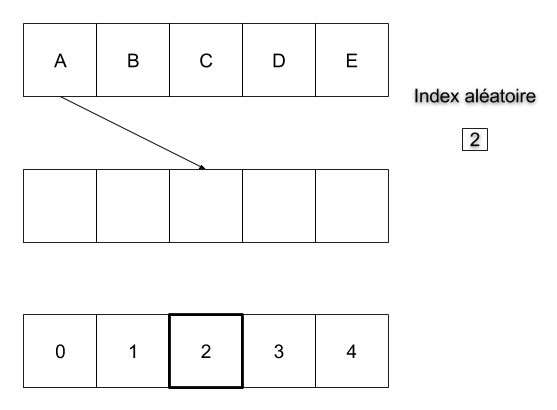
\includegraphics[width=0.3\textwidth]{rsc/index1_1.png}
                    \label{subfig:index1_1}}
                \subfloat[Itération 2]{
                    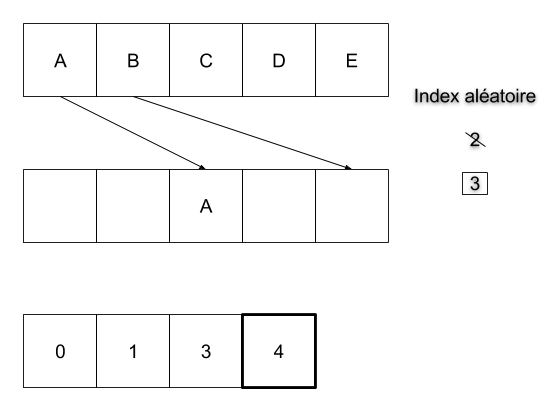
\includegraphics[width=0.3\textwidth]{rsc/index1_2.png}
                    \label{subfig:index1_2}}
                \subfloat[Itération 3]{
                    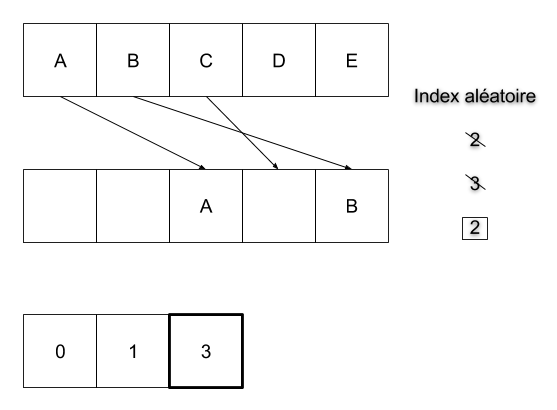
\includegraphics[width=0.3\textwidth]{rsc/index1_3.png}
                    \label{subfig:index1_3}}
                \caption{Choix pseudo-aléatoire des nouveaux indices des pixels}
                \label{fig:cipher}
            \end{center}
        \end{figure}

        Pour la première (cf. figure \ref{fig:cipher}\subref{subfig:index1_1}), le chiffre 2 est tiré par le générateur. Le nouvel indice du premier pixel de l'image sera donc 2. On supprime ensuite la $3^{eme}$ case du tableau d'indice (les indices commencent  à 0) et on recommence l'opération.
        Pour la deuxième itération (cf. figure \ref{fig:cipher}\subref{subfig:index1_2}), le chiffre 3 est tiré. La case d'indice 3 du taleau d'indice n'ayant plus la valeur 3 mais 4. Le deuxième pixel de l'image sera donc en case 5 de la nouvelle image.
        Pour ce qui est de la troisième itération (cf. figure \ref{fig:cipher}\subref{subfig:index1_3}), le chiffre 2 sort à nouveau. Cette fois ci, la troisième case du tableau d'indice contient la valeur 3. Le troisième pixel de l'image sera donc en position 4.

    \section{Algorithme de déchiffrement par permutation pseudo-aléatoire}

        L'algorithme de déchiffrement (cf. algorithme \ref{algo:decipher}) se base sur le même principe que celui de chiffrement. La différence repose sur l'ordre de parcours des tableaux. L'algorithme de chiffrement parcours dans l'ordre l'image d'entrée et dans le désordre l'image de sortie alors que l'algorithme de déchiffrement fait l'inverse. L'image chiffré est lu dans le désordre et l'image déchiffrée est écrite dans l'ordre.

        \begin{algorithm}[htbp]
            \SetAlgoLined
            \KwData{inputImage, cipherKey}
            \KwResult{outputImage}
            srand(cipherKey)\;
            size $\leftarrow$ height * width\;
            index $\leftarrow$ int[size]\;
            \For{i $\leftarrow$ 0 \KwTo size}{
                r $\leftarrow$ random(index.size())\;
                oldIndex $\leftarrow$ index[r]\;

                outputImageR[i] $\leftarrow$ inputImageR[oldIndex]\;
                outputImageG[i] $\leftarrow$ inputImageG[oldIndex]\;
                outputImageB[i] $\leftarrow$ inputImageB[oldIndex]\;

                index[r].remove()\;
            }
            \caption{Algorithme de chiffrement par permutation pseudo-aléatoire d'une image couleur}
            \label{algo:decipher}
        \end{algorithm}

        Selon le même procédé, la figure \ref{fig:decipher} montre les trois premières itérations pour le même tableau de cinq cases.

        \begin{figure}[htbp]
            \begin{center}
                \subfloat[Itération 1]{
                    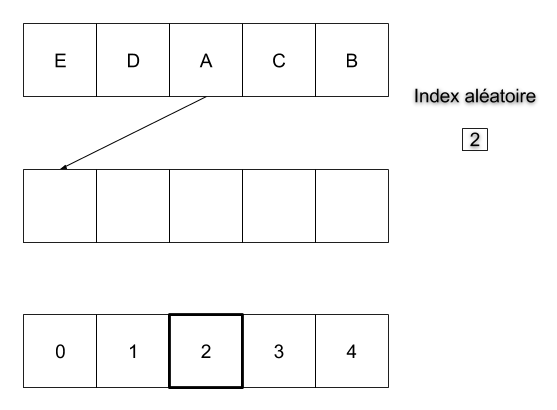
\includegraphics[width=0.3\textwidth]{rsc/index2_1.png}
                    \label{subfig:index2_1}}
                \subfloat[Itération 2]{
                    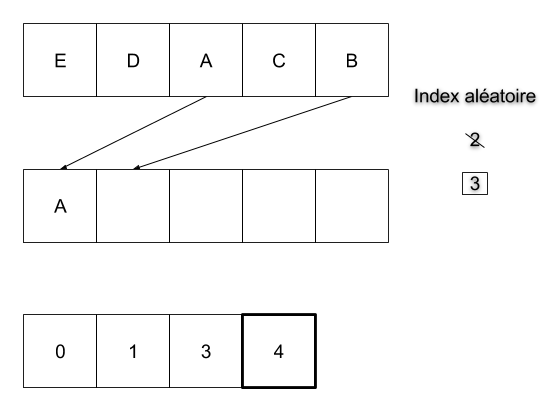
\includegraphics[width=0.3\textwidth]{rsc/index2_2.png}
                    \label{subfig:index2_2}}
                \subfloat[Itération 3]{
                    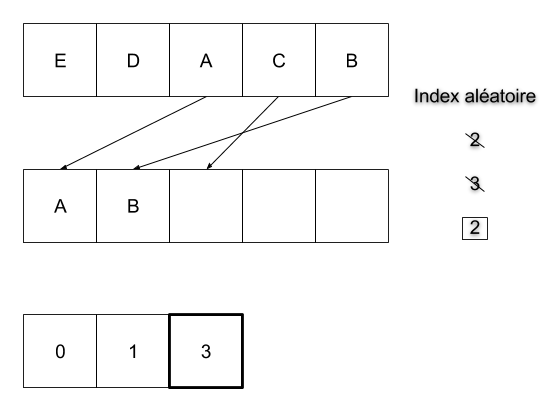
\includegraphics[width=0.3\textwidth]{rsc/index2_3.png}
                    \label{subfig:index2_3}}
                \caption{Récupération pseudo-aléatoire des anciens indices des pixels}
                \label{fig:decipher}
            \end{center}
        \end{figure}

        Les nombres tirés par le générateur pseudo-aléatoire apparaissent exactement dans le même ordre que lors du chiffrement (à condition que la clef renseignée soit la même également).
        Dans cette situation, on va donc chercher la valeur dans l'image d'entré à l'indice renseigné dans le tableau d'indice en fonction du nombre pseudo-aléatoire tiré. On va ensuite stocker cette valeur dans la prochaine case libre de l'image de sortie.

    \section{Permutation par blocs}

        Afin de permettre à un appareil photo de récupérer et réorganiser correctement tous les pixels il faut les agencer et les déplacer par blocs entiers. Il faut donc ajouter aux algorithmes précédents un deuxième groupe de boucle pour les blocs.

        \begin{algorithm}[htbp]
            \SetAlgoLined
            \KwData{inputImage, cipherKey}
            \KwResult{outputImage}
            srand(cipherKey)\;
            size $\leftarrow$ height * width\;
            index $\leftarrow$ int[size]\;
            \For{i $\leftarrow$ 0 \KwTo size}{
                r $\leftarrow$ random(index.size())\;
                newIndexBlock $\leftarrow$ index[r]\;
                oldIndexFirst = (i - (mod(i, nbBlockWidth))) * sizeBlock + ((mod(i, nbBlockWidth)) * widthBlock)\;
                newIndexFirst = (newBlockIndex - (mod(newBlockIndex, nbBlockWidth))) * sizeBlock + ((mod(newBlockIndex, nbBlockWidth)) * widthBlock)\;

                \For{x $\leftarrow$ 0 \KwTo widthBlock}{
                    \For{y $\leftarrow$ 0 \KwTo widthBlock}{
                        newIndex = newIndexFirst + x + (y * width)\;
                        oldIndex = oldIndexFirst + x + (y * width)\;

                        outputImageR[newIndex] $\leftarrow$ inputImageR[oldIndex]\;
                        outputImageG[newIndex] $\leftarrow$ inputImageG[oldIndex]\;
                        outputImageB[newIndex] $\leftarrow$ inputImageB[oldIndex]\;
                    }
                }
            }
            \caption{Algorithme de chiffrement par permutation pseudo-aléatoire d'une image couleur}
            \label{algo:cipher_block}
        \end{algorithm}

        Dans l'algorithme \ref{algo:cipher_block}, la première boucle gère les différents blocs comme un pixel simple et calcule les coordonnées de l'angle supérieur gauche des blocs de départ et d'arrivé. La seconde section de boucle permet de calculer directement les coordonnées des pixels du bloc.

    \section{Moyenne des pixels}

        Dans le même intérêt de faciliter la récupération des images par un appareil photo, on peut remplacer chaque pixel d'un bloc par une même valeur. On peut par exemple calculer la moyenne des pixels du bloc puis l'appliquer à tous les pixels de ce bloc avant de les déplacer.

    \section{Résultats}

        \subsection{Chiffrement}

            Les résultats des algorithmes de chiffrement sont présentés dans les figures \ref{fig:res_picasso} et \ref{fig:res_vangogh}.

            Les figures :
            \begin{itemize}
                \item \subref{subfig:picasso_original} montrent les images d'origines utilisé pour les tests
                \item \subref{subfig:picasso_pixels} montrent les images chiffrées par les pixels
                \item \subref{subfig:picasso_10}, \subref{subfig:picasso_25} et \subref{subfig:picasso_50} montrent les images chiffrées avec respectivement 10, 25 et 50 blocs
                \item \subref{subfig:picasso_10_a}, \subref{subfig:picasso_25_a} et \subref{subfig:picasso_50_a} montrent les images chiffrées avec respectivement 10, 25 et 50 blocs avec la moyenne des blocs.
            \end{itemize}

            \begin{figure}[htbp]
                \begin{center}
                    \subfloat[Picasso]{
                        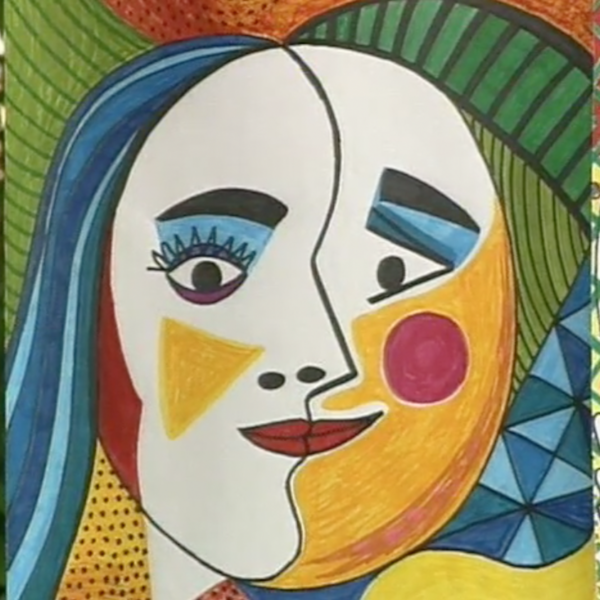
\includegraphics[width=0.3\textwidth]{rsc/picasso.png}
                        \label{subfig:picasso_original}}
                    \subfloat[Permutation par pixels]{
                        
\includegraphics[width=0.3\textwidth]{rsc/picasso_600_12.png}
                        \label{subfig:picasso_pixels}}\\
                    \subfloat[Permutation 10 blocs]{
                        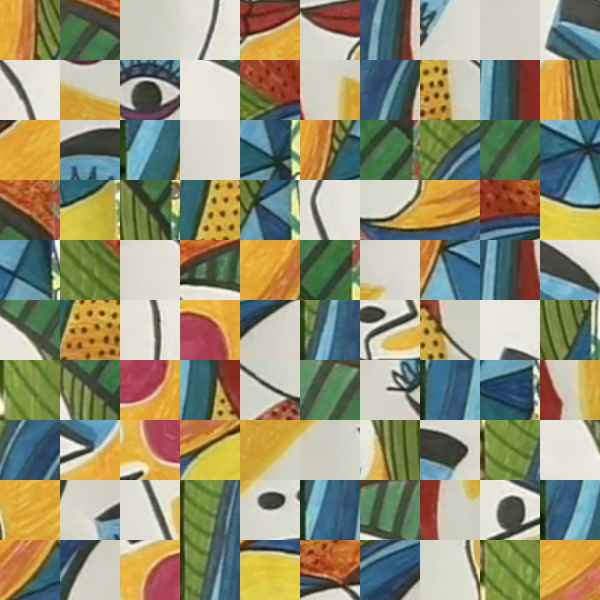
\includegraphics[width=0.3\textwidth]{rsc/picasso_10_12.png}
                        \label{subfig:picasso_10}}
                    \subfloat[Permutation 25 blocs]{
                        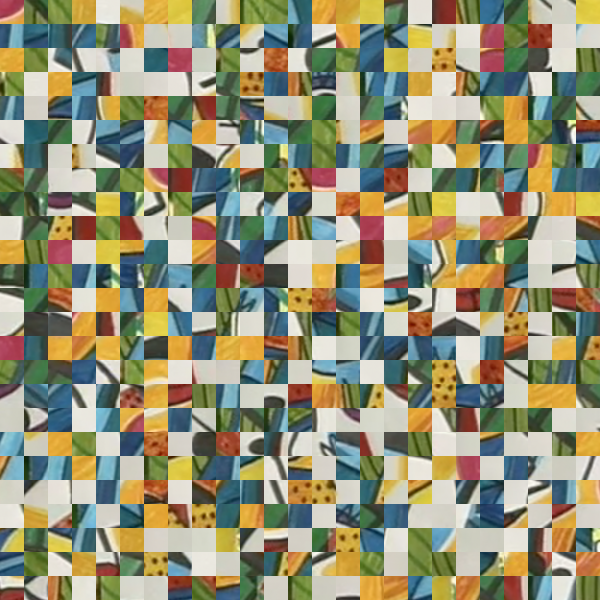
\includegraphics[width=0.3\textwidth]{rsc/picasso_25_12.png}
                        \label{subfig:picasso_25}}
                    \subfloat[Permutation 50 blocs]{
                        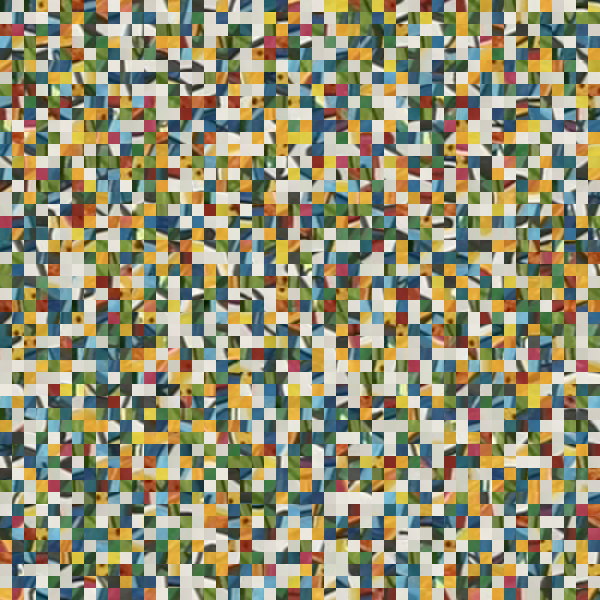
\includegraphics[width=0.3\textwidth]{rsc/picasso_50_12.png}
                        \label{subfig:picasso_50}}\\
                    \subfloat[Permutation 10 blocs moyennés]{
                        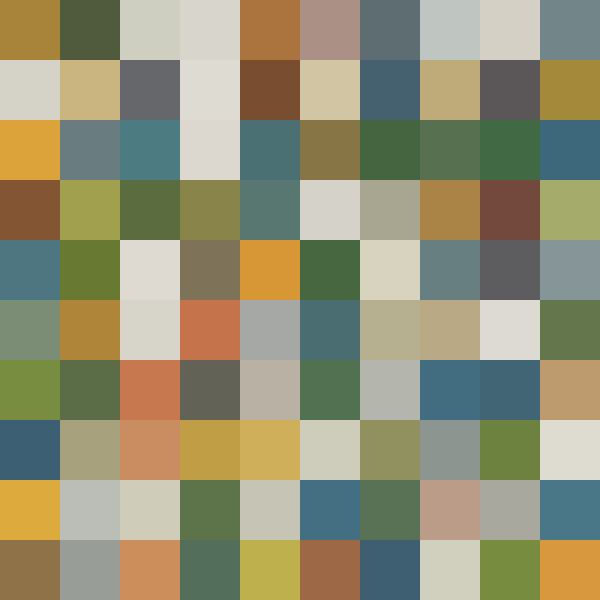
\includegraphics[width=0.3\textwidth]{rsc/picasso_a_10_12.png}
                        \label{subfig:picasso_10_a}}
                    \subfloat[Permutation 25 blocs moyennés]{
                        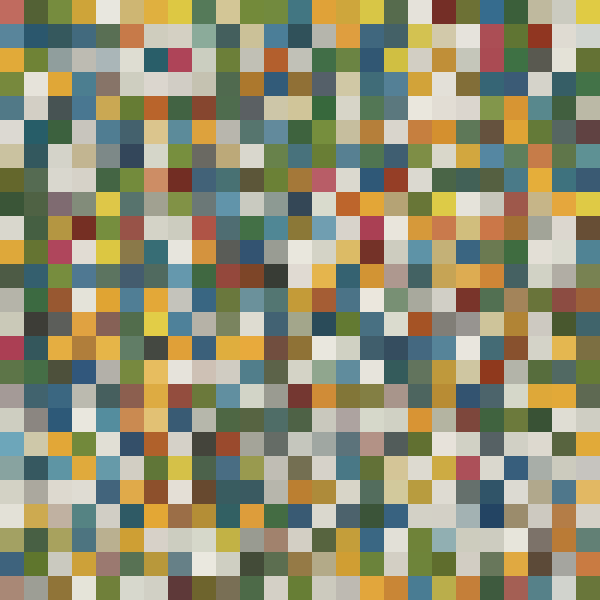
\includegraphics[width=0.3\textwidth]{rsc/picasso_a_25_12.png}
                        \label{subfig:picasso_25_a}}
                    \subfloat[Permutation 50 blocs moyennés]{
                        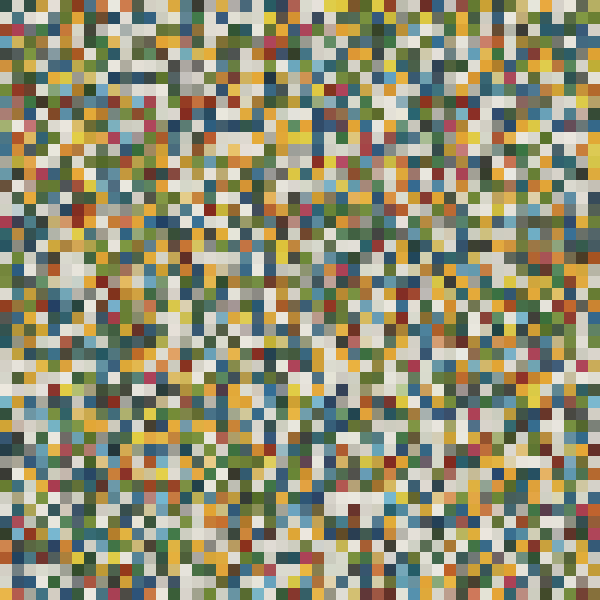
\includegraphics[width=0.3\textwidth]{rsc/picasso_a_50_12.png}
                        \label{subfig:picasso_50_a}}
                    \caption{Résultat du chiffrement de la peinture "Picasso" par pixels et par blocs}
                    \label{fig:res_picasso}
                \end{center}
            \end{figure}

            \begin{figure}[htbp]
                \begin{center}
                    \subfloat[Van Gogh]{
                        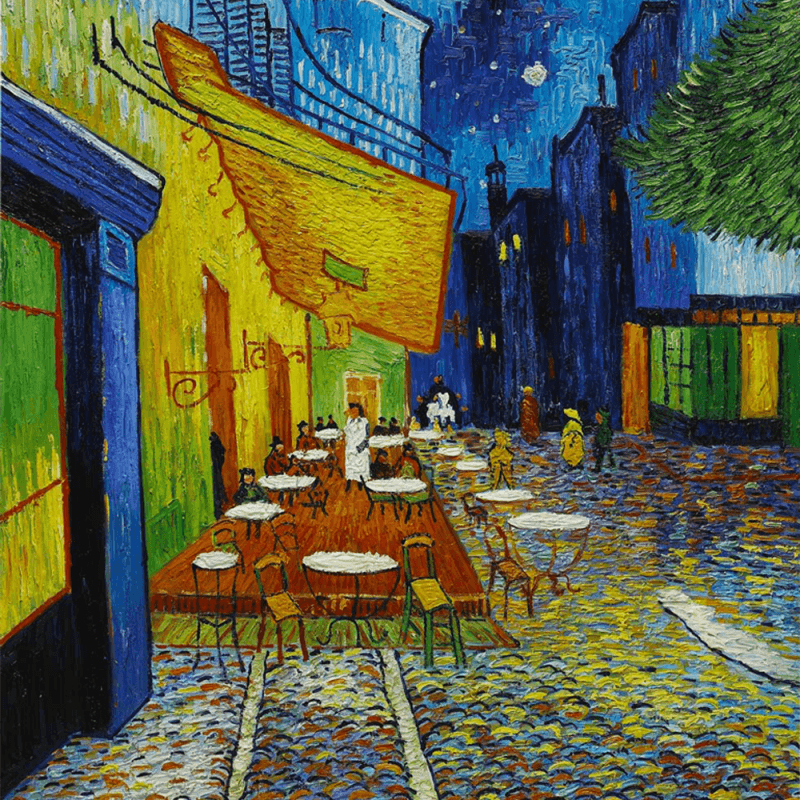
\includegraphics[width=0.3\textwidth]{rsc/van_gogh.png}
                        \label{subfig:vangogh_original}}
                    \subfloat[Permutation par pixels]{
                        
\includegraphics[width=0.3\textwidth]{rsc/van_gogh_800_12.png}
                        \label{subfig:vangogh_pixels}}\\
                    \subfloat[Permutation 10 blocs]{
                        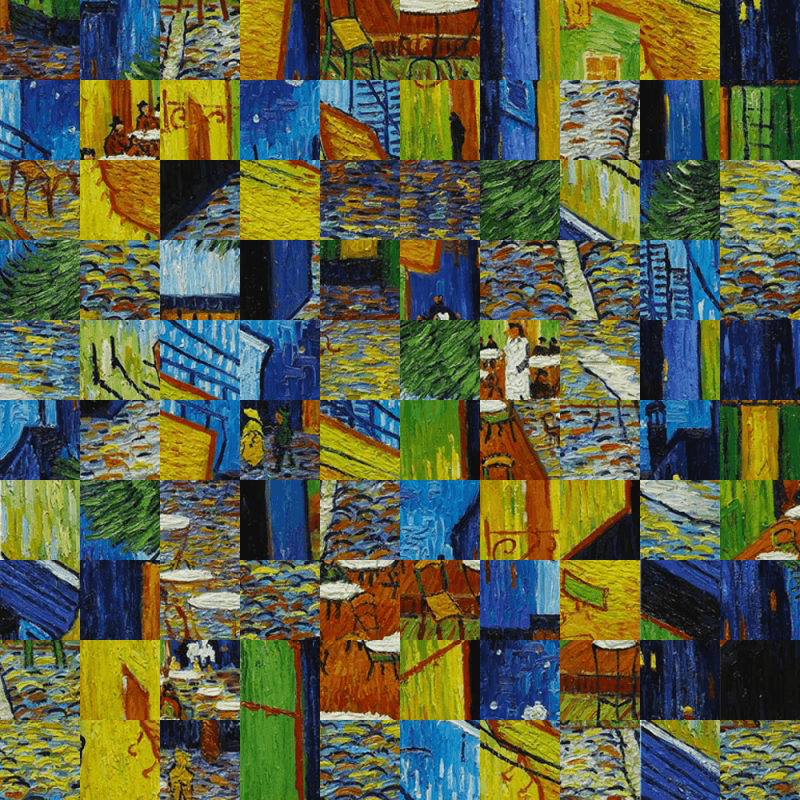
\includegraphics[width=0.3\textwidth]{rsc/van_gogh_10_12.png}
                        \label{subfig:vangogh_10}}
                    \subfloat[Permutation 25 blocs]{
                        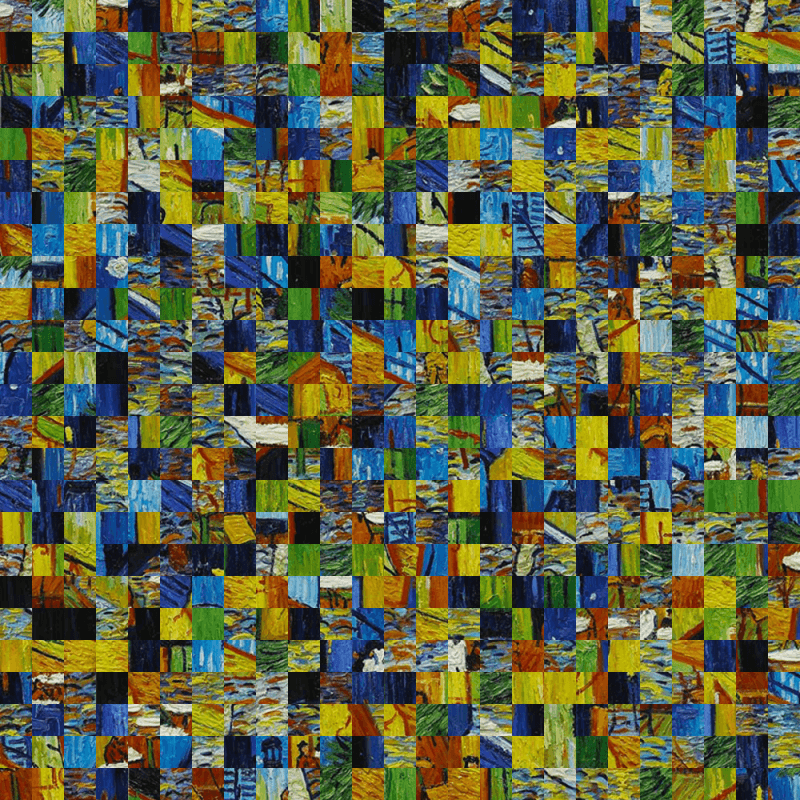
\includegraphics[width=0.3\textwidth]{rsc/van_gogh_25_12.png}
                        \label{subfig:vangogh_25}}
                    \subfloat[Permutation 50 blocs]{
                        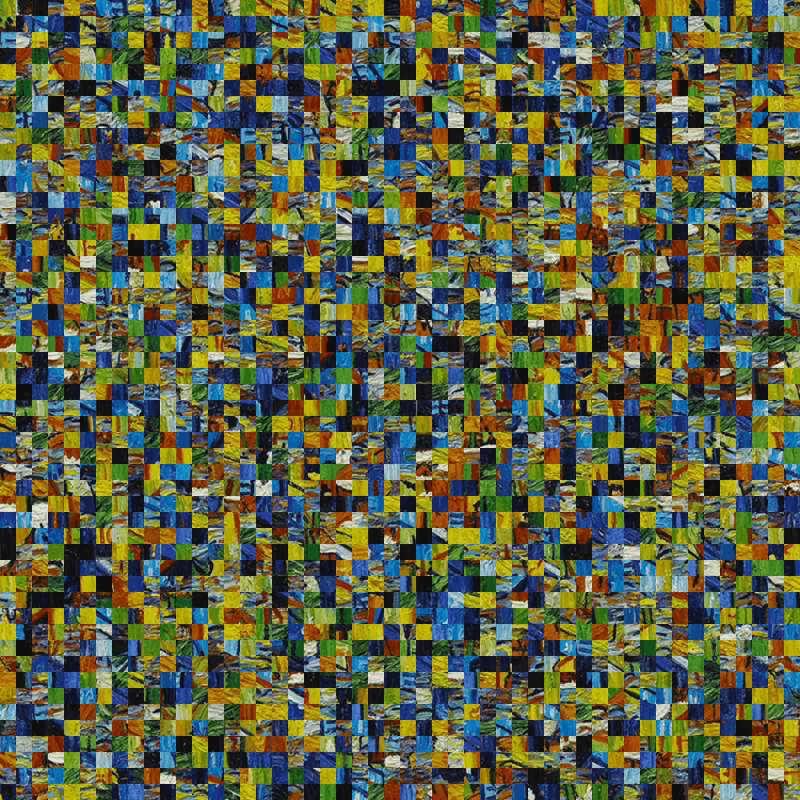
\includegraphics[width=0.3\textwidth]{rsc/van_gogh_50_12.png}
                        \label{subfig:vangogh_50}}\\
                    \subfloat[Permutation 10 blocs moyennés]{
                        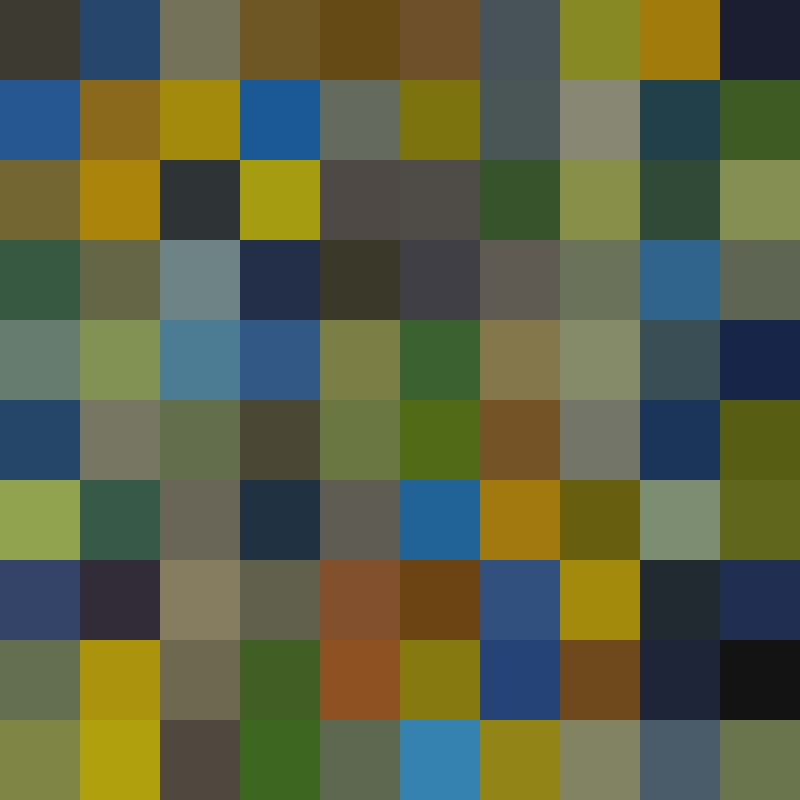
\includegraphics[width=0.3\textwidth]{rsc/van_gogh_a_10_12.png}
                        \label{subfig:vangogh_10_a}}
                    \subfloat[Permutation 25 blocs moyennés]{
                        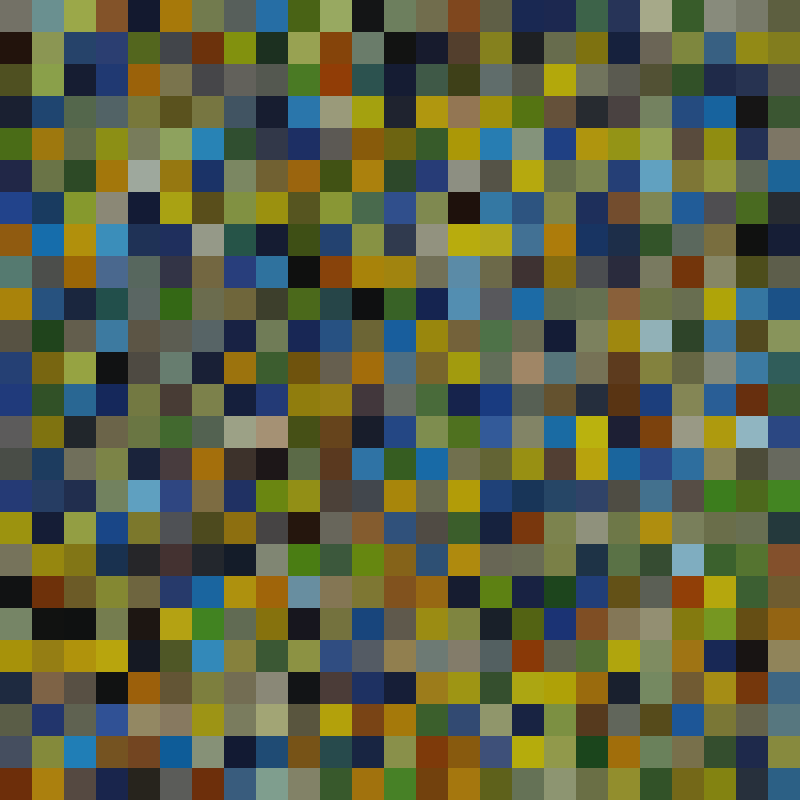
\includegraphics[width=0.3\textwidth]{rsc/van_gogh_a_25_12.png}
                        \label{subfig:vangogh_25_a}}
                    \subfloat[Permutation 50 blocs moyennés]{
                        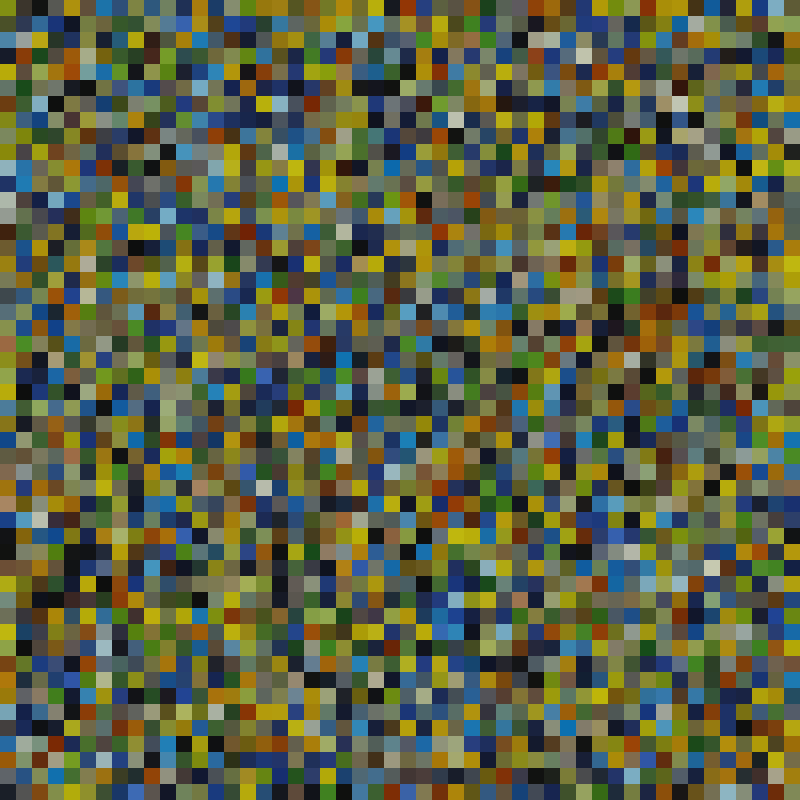
\includegraphics[width=0.3\textwidth]{rsc/van_gogh_a_50_12.png}
                        \label{subfig:vangogh_50_a}}
                    \caption{Résultat du chiffrement de la peinture "Van Gogh" par pixels et par blocs}
                    \label{fig:res_vangogh}
                \end{center}
            \end{figure}

        \subsection{Déchiffrement}

            Le déchiffrement des images \subref{subfig:picasso_pixels}, \subref{subfig:picasso_10}, \subref{subfig:picasso_25} et \subref{subfig:picasso_50} permet de récupérer les images originales.

            Quant au déchiffrement des images \subref{subfig:picasso_10_a}, \subref{subfig:picasso_25_a} et \subref{subfig:picasso_50_a}, il renvoie les image (respectivement) \ref{fig:res_average}\subref{subfig:picasso_a_10}, \ref{fig:res_average}\subref{subfig:picasso_a_25}, \ref{fig:res_average}\subref{subfig:picasso_a_50} et \ref{fig:res_average}\subref{subfig:vangogh_a_10}, \ref{fig:res_average}\subref{subfig:vangogh_a_25}, \ref{fig:res_average}\subref{subfig:vangogh_a_50} et

            \begin{figure}[htbp]
                \begin{center}
                    \subfloat[Picasso 10 blocs moyennés]{
                        
\includegraphics[width=0.3\textwidth]{rsc/picasso_a_10_12_d.png}
                        \label{subfig:picasso_a_10}}
                    \subfloat[Picasso 25 blocs moyennés]{
                        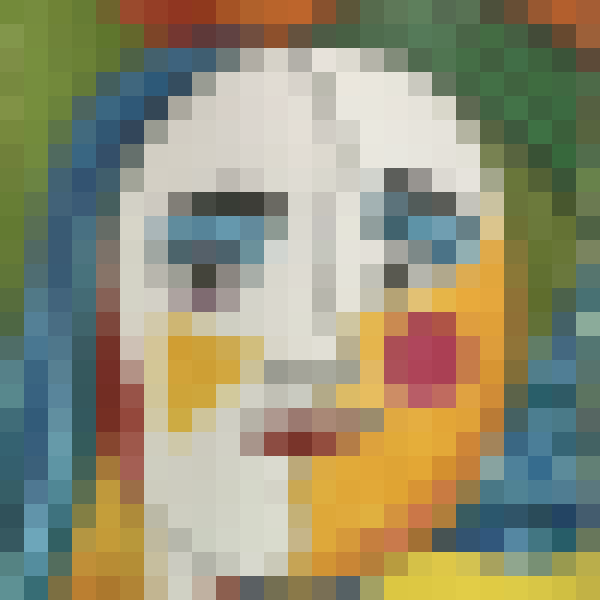
\includegraphics[width=0.3\textwidth]{rsc/picasso_a_25_12_d.png}
                        \label{subfig:picasso_a_25}}
                    \subfloat[Picasso 50 blocs moyennés]{
                        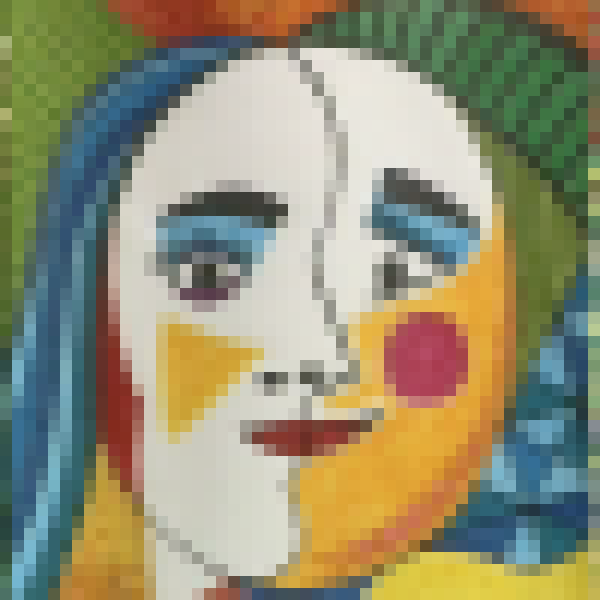
\includegraphics[width=0.3\textwidth]{rsc/picasso_a_50_12_d.png}
                        \label{subfig:picasso_a_50}}\\
                    \subfloat[Van Gogh 10 blocs moyennés]{
                        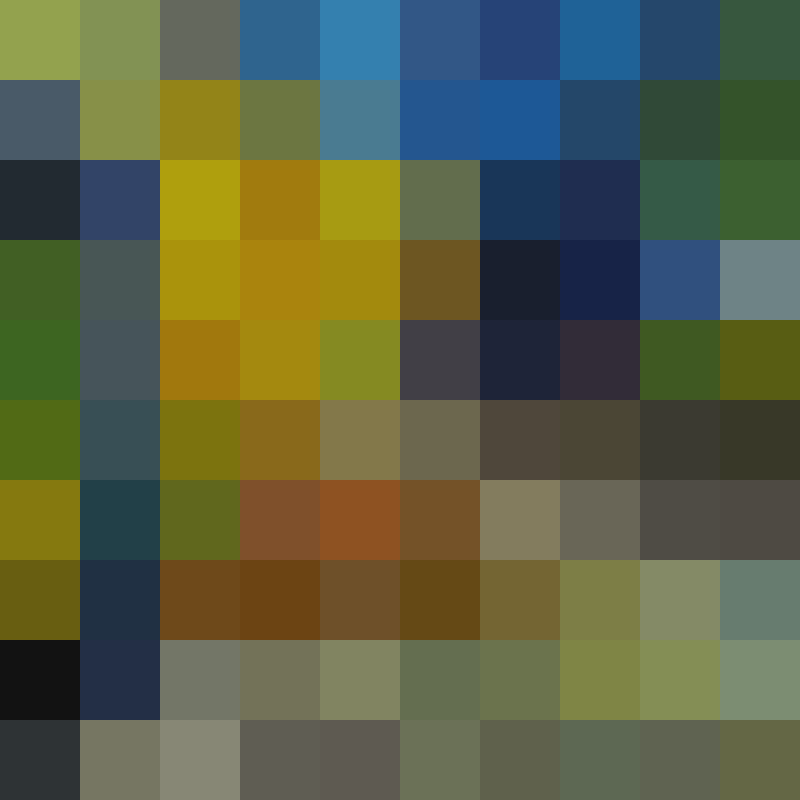
\includegraphics[width=0.3\textwidth]{rsc/van_gogh_a_10_12_d.png}
                        \label{subfig:vangogh_a_10}}
                    \subfloat[Van Gogh 25 blocs moyennés]{
                        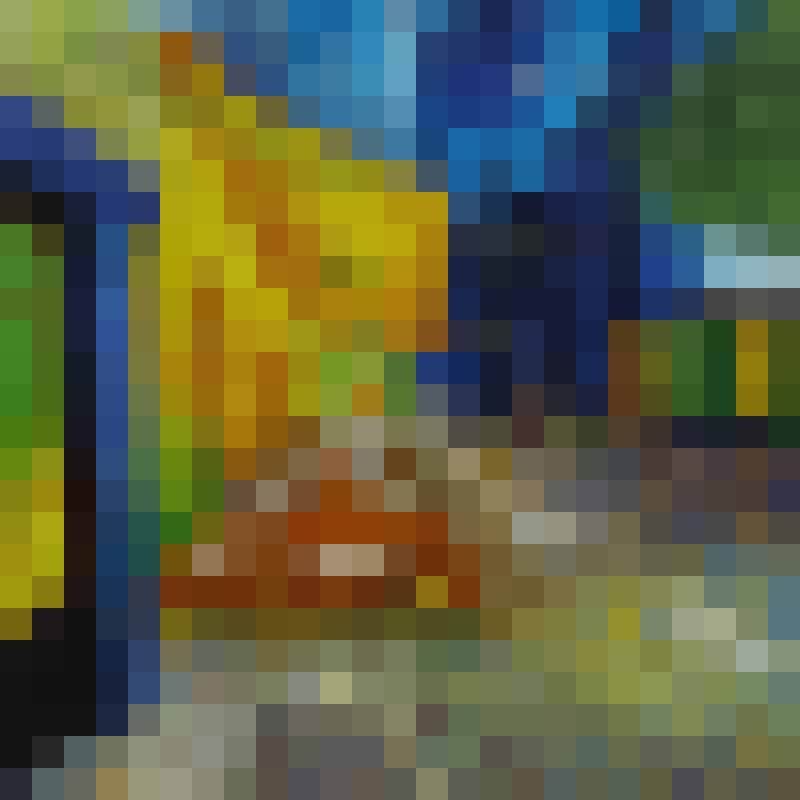
\includegraphics[width=0.3\textwidth]{rsc/van_gogh_a_25_12_d.png}
                        \label{subfig:vangogh_a_25}}
                    \subfloat[Van Gogh 50 blocs moyennés]{
                        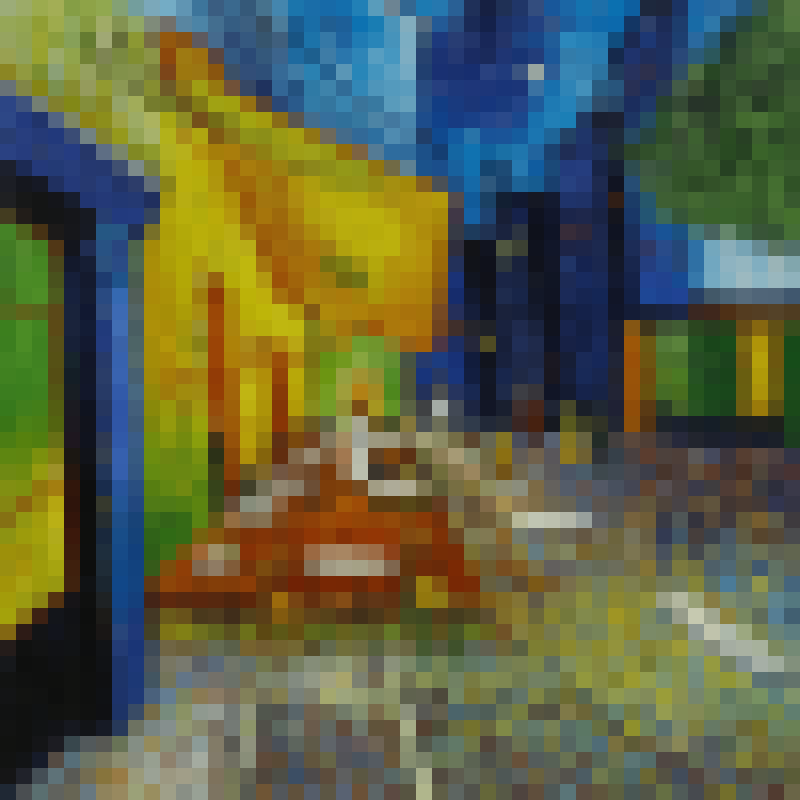
\includegraphics[width=0.3\textwidth]{rsc/van_gogh_a_50_12_d.png}
                        \label{subfig:vangogh_a_50}}
                    \caption{Résultat du déchiffrement des peintures "Picasso" et "Van Gogh" par blocs avec moyenne}
                    \label{fig:res_average}
                \end{center}
            \end{figure}

\end{document}
